\documentclass[11pt]{article}

% Paquetes
%===============================================================================

% Establecemos los márgenes
\usepackage[a4paper, margin=1in]{geometry}

% Separacion entre parrafos
\setlength{\parskip}{1em}

% Paquete para incluir codigo
\usepackage{listings}
\usepackage{listings-rust}

% Paquete para incluir imagenes
\usepackage{graphicx}
\graphicspath{ {./images/} }

% Para fijar las imagenes en la posicion deseada
\usepackage{float}

% Para que el codigo acepte caracteres en utf8
\lstset{literate=
  {á}{{\'a}}1 {é}{{\'e}}1 {í}{{\'i}}1 {ó}{{\'o}}1 {ú}{{\'u}}1
  {Á}{{\'A}}1 {É}{{\'E}}1 {Í}{{\'I}}1 {Ó}{{\'O}}1 {Ú}{{\'U}}1
  {à}{{\`a}}1 {è}{{\`e}}1 {ì}{{\`i}}1 {ò}{{\`o}}1 {ù}{{\`u}}1
  {À}{{\`A}}1 {È}{{\'E}}1 {Ì}{{\`I}}1 {Ò}{{\`O}}1 {Ù}{{\`U}}1
  {ä}{{\"a}}1 {ë}{{\"e}}1 {ï}{{\"i}}1 {ö}{{\"o}}1 {ü}{{\"u}}1
  {Ä}{{\"A}}1 {Ë}{{\"E}}1 {Ï}{{\"I}}1 {Ö}{{\"O}}1 {Ü}{{\"U}}1
  {â}{{\^a}}1 {ê}{{\^e}}1 {î}{{\^i}}1 {ô}{{\^o}}1 {û}{{\^u}}1
  {Â}{{\^A}}1 {Ê}{{\^E}}1 {Î}{{\^I}}1 {Ô}{{\^O}}1 {Û}{{\^U}}1
  {ã}{{\~a}}1 {ẽ}{{\~e}}1 {ĩ}{{\~i}}1 {õ}{{\~o}}1 {ũ}{{\~u}}1
  {Ã}{{\~A}}1 {Ẽ}{{\~E}}1 {Ĩ}{{\~I}}1 {Õ}{{\~O}}1 {Ũ}{{\~U}}1
  {œ}{{\oe}}1 {Œ}{{\OE}}1 {æ}{{\ae}}1 {Æ}{{\AE}}1 {ß}{{\ss}}1
  {ű}{{\H{u}}}1 {Ű}{{\H{U}}}1 {ő}{{\H{o}}}1 {Ő}{{\H{O}}}1
  {ç}{{\c c}}1 {Ç}{{\c C}}1 {ø}{{\o}}1 {å}{{\r a}}1 {Å}{{\r A}}1
  {€}{{\euro}}1 {£}{{\pounds}}1 {«}{{\guillemotleft}}1
  {»}{{\guillemotright}}1 {ñ}{{\~n}}1 {Ñ}{{\~N}}1 {¿}{{?`}}1 {¡}{{!`}}1
}

% Para que no se salgan las lineas de codigo
\lstset{breaklines=true}

% Para que los metadatos que escribe latex esten en español
\usepackage[spanish]{babel}

% Para la bibliografia
% Sin esto, los enlaces de la bibliografia dan un error de compilacion
\usepackage{url}

% Para mostrar graficas de dos imagenes, cada una con su caption, y con un caption comun
\usepackage{subcaption}

% Simbolo de los numeros reales
\usepackage{amssymb}

% Para que los codigos tengan una fuente distinta
\usepackage{courier}

% TODO -- bajar el tamaño de la fuente
\lstdefinestyle{CustomStyle}{
  language=Python,
  numbers=left,
  stepnumber=1,
  numbersep=10pt,
  tabsize=4,
  showspaces=false,
  showstringspaces=false
  basicstyle=\tiny\ttfamily,
}

% Para incluir tablas en csv
\usepackage{csvsimple}

% Para referenciar secciones usando el nombre de las secciones
\usepackage{nameref}

% Para enumerados dentro de enumerados
\usepackage{enumitem}

% Metadatos del documento
%===============================================================================
\title{
{Práctica 2b}\\
{Técnicas de Búsqueda Basadas en Poblaciones}\\
{Problema de Agrupamiento con Restricciones}\\
}
\author{
{Sergio Quijano Rey - 72103503k}\\
{4º Doble Grado Ingeniería Informática y Matemáticas}\\
{Grupo de prácticas 2 - Viernes 17.30h a 19.30h}\\
{sergioquijano@correo.ugr.es}
}
\date{\today}

% Contenidos del documento
%===============================================================================

\begin{document}

% Portada del documento
\maketitle
\pagebreak

% % Indice de contenidos
\tableofcontents

% Lista de figuras
\listoffigures

% Referencias bibliográficas
\bibliography{References}
\bibliographystyle{ieeetr}

\pagebreak

\section{Descripción del problema}

Vamos a trabajar el problema del agrupamiento con restricciones (\textbf{\emph{PAR}}). Consiste en una generalización del problema de agrupamiento clásico, al que añadimos restricciones sobre los datos.

El problema de agrupamiento clásico consiste en, dados unos datos de entrada sin etiquetar $X$ de tamaño $n$, agruparlos en $k$ grupos (o en inglés, \emph{clusters}) diferentes, formando una partición $C$ de $X$, de forma que se optimice alguna métrica. Normalmente, se busca minimizar la distancia \emph{intra\_cluster} (que más tarde se definirá).

La diferencia con el problema de agrupamiento clásico, por tanto, es la inclusión de restricciones. En nuestro caso concreto, trabajemos con restricciones entre pares de puntos, que además serán de dos tipos:

\begin{itemize}
\item Restricción tipo \emph{Must Link}: los dos puntos afectados por esta restricción deberán pertenecer al mismo cluster
\item Restricción tipo \emph{Cannot Link}: los dos puntos afectados por esta restricción no deben pertenecer al mismo cluster
\end{itemize}

Consideraremos de forma débil estas restricciones, es decir, podemos incumplir algunas restricciones. Pero supondrá que la solución será de peor calidad. Para especificar mejor esta noción, definimos la función de \emph{fitness} que buscamos minimizar:

\begin{displaymath}
fitness(sol) := distancia_{intra-cluster}(sol) + \lambda * infeasibility(sol)
\end{displaymath}

donde $infeasibility$ es el número de restricciones que se incumplen. Esta función de $fitness$ nos permite pasar de intentar optimizar dos funciones objetivo a solo tener que optimizar un objetivo. El valor de $\lambda$ se especifica más adelante.

Como los datos no están etiquetados a priori, podríamos considerar este problema como un problema de aprendizaje no supervisado. Sin embargo, se puede considerar que las restricciones nos dan un tipo de etiquetado, por lo que es más correcto pensar que estamos ante una tarea de aprendizaje \emph{semi-supervisado}. La principal utilidad de resolver estos problemas es que normalmente estamos reduciendo la dimensionalidad de los datos a analizar, y de este modo, es más sencillo extraer conocimiento sobre dichos datos.

\pagebreak

\section{Descripción de la aplicación de los algoritmos empleados}

\subsection{Representación del conjunto de datos}

Los datos vienen dados en una matriz de tamaño $n \times d$ donde $n$ es el número de puntos y $d$ es la dimensión de cada uno de los puntos.

\subsubsection{Representación del conjunto de datos en código}

El conjunto de datos viene representado en \lstinline{problem_datatypes::DataPoints} que contiene un vector de otro tipo de dato: \lstinline{problem_datatypes::Point}. El tipo de dato \lstinline{Point} tiene un campo que es de tipo \lstinline{ndarray::Array1<f64>} que representa un vector (usamos una librería para trabajar con matrices y vectores). Por tanto, hemos pasado de trabajar con una matriz de datos a trabajar con un vector de puntos. Esto nos permite trabajar de forma más expresiva y sencilla con el problema. Por ejemplo, podemos calcular con métodos del \lstinline{struct} distancia entre dos puntos, centroide de un conjunto de puntos, \ldots

\subsection{Representación de las restricciones}

Las restricciones vienen dadas en un fichero de datos que representa una matriz que codifica las restricciones de la siguiente forma:

\begin{itemize}
\item El elemento en la fila $i$-ésima y columna $j$-ésima representa las restricciones que hay entre el punto $i$ y el punto $j$
\item Como la restricción que tenga el punto $i$ con el punto $j$ implica que el punto $j$ tiene la misma restricción con el punto $i$, es claro que dicha matriz debe ser simétrica
\item Un valor $0$ significa que no hay restricciones. Un valor $1$ significa que hay una restricción tipo \emph{Must Link}. Un valor $-1$ implica una restricción \emph{Cannot Link}
\item Además, la matriz tiene la diagonal de $1$s
\end{itemize}

\subsubsection{Representación de las restricciones en código}

El \lstinline{struct} \lstinline{problem_datatypes::Constraints} junto al enumerado \lstinline{problem_datatypes::ConstraintType} representan en el código las restricciones. El código es el siguiente:

\begin{lstlisting}[language=Rust, style=Boxed]
pub enum ConstraintType {
MustLink,
CannotLink,
}

pub struct Constraints{
data: HashMap<(i32, i32), ConstraintType>,
}
\end{lstlisting}

Es claro que guardamos pares de enteros, que marcan los índices de los puntos, y la restricción entre el par de puntos representados, en un \lstinline{HashMap}. Esta elección viene motivada por:

\begin{itemize}
\item Podemos acceder a las restricciones entre dos puntos en tiempo constante
\item Podemos iterar sobre todas las restricciones, gracias a los métodos proporcionados por el lenguaje de programación, en un tiempo más que razonable. Así iteramos solo sobre una lista de $r$ restricciones, en vez de sobre una matriz cuadrada de dimensión $n^2$
\item En cierto modo, estamos combinando los beneficios de tener acceso directo a elementos concretos y los beneficios de poder iterar sobre una lista (aunque iterar sobre un \lstinline{Hash} puede ser algo más lento que iterar sobre una lista o un \lstinline{array})
\item Es fácil de implementar métodos para operar con restricciones con este tipo de dato
\end{itemize}

La implementación de los métodos que permiten manipular el \lstinline{struct} aseguran que:
\begin{itemize}
\item No guardamos la restricción $(i, j)$ y junto a la $(j, i)$. Solo guardamos una de las dos restricciones, ahorrando memoria
\item De hecho, el criterio es guardar como índices el par $(i, j)$ donde $i \leq j$
\item Tampoco guardamos las restricciones $(i, i), MustLink$ pues son restricciones triviales
\end{itemize}


\subsection{Representación de la solución}

Una representación de la solución será un vector de tamaño $n$ con valores en $\{0, \ldots, k - 1\}$ donde $n$ es el número de puntos y $k$ es el número de clusters en los que dividimos los datos. Este vector representa la partición de los datos en los $k$ clusters. En la posición $i$-ésima del vector, guardamos el cluster al que pertenece el punto $i$-ésimo de nuestro conjunto de datos.

Las soluciones deben cumplir las siguientes restricciones:

\begin{itemize}
\item No pueden quedar clusters vacíos. Es decir, clusters a los que no haya ningún punto asignado. Esto puede verse viendo que $\forall i \in \{0, \ldots, k-1\}$ $\exists pos \in \{0, \ldots, n-1\}$ tal que $solution[pos] = i$, es decir, el vector de soluciones tiene al menos una vez cada valor posible de los clusters
\item Cada punto solo puede pertenecer a un único cluster. Por la forma vectorial en la que representamos la partición, esta restricción se verifica forzosamente, y por tanto no nos tenemos que preocupar de realizar comprobaciones
\item La unión de los puntos de los clusters debe ser todo el conjunto de datos, es decir, $X = \bigcup c_i$. De nuevo, nuestra representación vectorial fuerza a que esta restricción se verifique
\end{itemize}

Por ejemplo, si tenemos 5 puntos y 3 clusters, una posible solución sería $\{3, 1, 2, 3, 0\}$. Y por otro lado, la solución $\{3, 1, 2, 3, 2\}$ no es válida pues el cluster $0$ está vacío.

Para cada solución podemos calcular algunas métricas necesarias para conocer el valor de $fitness$ de la solución que estamos representando. Para comenzar, por cada cluster podemos calcular el \textbf{centroide} del cluster:

\begin{displaymath}
\vec{\mu_i} := \frac{1}{|c_i|} \sum_{x_i \in c_i} \vec{x_i}
\end{displaymath}

Definimos para cada cluster su \textbf{distancia media intra-cluster} como:

\begin{displaymath}
\bar{c_i} := \frac{1}{|c_i|} \sum_{x_i \in c_i} || \vec{x_i} - \vec{\mu_i} ||_2
\end{displaymath}

Y con ello podemos definir la \textbf{desviación general de la partición} como:

\begin{displaymath}
\bar{c} := \frac{1}{k} \sum_{i \in 1, \ldots k} \bar{c_i}
\end{displaymath}

Definimos $infeasibility$ como el número de restricciones, tanto del tipo \emph{Must Link} como del tipo \emph{Cannot Link}, que se violan.

Con ello, ya podemos definir el valor de $\lambda$ como $\lambda := \frac{D}{|R|}$ donde $|R|$ es el número total de restricciones y $D$ la distancia máxima entre dos puntos de $X$.

Cuando trabajemos con algoritmos poblacionales, usaremos la siguiente \textbf{nomenclatura}:

\begin{itemize}
    \item Población: conjunto de soluciones
    \item Cromosoma: una solución individual
    \item Gen: cada uno de los elementos del vector de asignación punto $\rightarrow$ cluster que compone la solución
\end{itemize}

\subsubsection{Representación de la solución en código}

La solución se representa en la clase \lstinline{problem_datatypes::Solution}. El código de los campos del \lstinline{struct} desarrollado es:

\begin{lstlisting}[language=Rust, style=Boxed]
pub struct Solution<'a, 'b> {
cluster_indexes: Vec<u32>,
data_points: &'a DataPoints,
constraints: &'b Constraints,
number_of_clusters: i32,

/// Representa el peso de infeasibility en el calculo de fitness
/// Solo se calcula una vez al invocar a Solution::new
lambda: f64,

// Para cachear el valor de fitness pues es un calculo costoso de realizar
// Como los datos del struct no cambian, podemos hacer el cacheo sin miedo
// Usamos RefCell para tener un patron de mutabilidad interior
fitness: RefCell<Option<f64>>,
}
\end{lstlisting}

Los campos del \lstinline{struct} representan:

\begin{itemize}
\item \lstinline{cluster_indixes}: el vector solución que representa la asignación de puntos a clusters
\item \lstinline{data_points}: referencia al conjunto de datos (sirve para calcular métricas como el $fitness$ de la solución que se representa)
\item \lstinline{constraints}: referencia al conjunto de restricciones sobre los datos (sirve para calcular métricas como el $fitness$ de la solución que se representa)
\item \lstinline{number_of_clusters}: número de clusters en los que se agrupan los datos (sirve para comprobar que una solución sea válida)
\item \lstinline{lambda}: valor de $\lambda$, necesario para calcular el $fitness$
\item \lstinline{fitness}: valor de $fitness$. Está incluida en un \lstinline{RefCell<Option<f64>>} para poder cachear su valor, puesto que los atributos de una instancia nunca cambian y el cálculo del valor $\lambda$ es muy costoso (implica calcular restricciones violadas y distancias entre puntos)
\end{itemize}

La comprobación de que no tenemos clusters sin puntos asignados se hace en el método \lstinline{Solution::is_valid}. La distancia media intracluster se calcula en \lstinline{Solution::intra_cluster_distance}. Mientras que la desviación general se calcula en \lstinline{Solution::global_cluster_mean_distance}. El valor de $infeasibility$ se calcula en \lstinline{Solution::infeasibility}. El cálculo de $\lambda$ se realiza en el \emph{constructor} del \lstinline{struct}.

Además, en todos los algoritmos, salvo \lstinline{copkmeans}, debemos llevar la cuenta de las evaluaciones de \emph{fitness} que consumimos. Para ello tenemos la función \lstinline{fitness_and_consumed}. También tenemos funciones para invalidar la cache, para comprobar si tenemos el \emph{fitness} cacheado o no, $\ldots$

\subsubsection{FitnessEvaluationResult}

Para mejorar el control sobre las evaluaciones del fitness, disponemos del struct  \lstinline{FitnessEvaluationResult<T>}. Guarda un tipo genérico \lstinline{T} y las evaluaciones que consume la operación que genera dicho valor. Por ejemplo, si en un población (de la que hablaremos más adelante), queremos encontrar el individuo con mejor valor de fitness, devolvemos \lstinline{FitnessEvaluationResult<Solution>} con dicho mejor individuo y las consumiciones de fitness \textbf{efectivas} que consume esta búsqueda.

\subsection{Representación de la población}

Una población, intuitivamente, es un conjunto de individuos, que en nuestro caso, serán soluciones válidas del problema que estamos intentando resolver. En código la representaremos como un vector de \lstinline{Solution}. Sobre este \lstinline{struct} podemos realizar operaciones comunes a los algoritmos genéticos, tanto generacionales como estacionarios, y a los algoritmos meméticos. Operaciones como generar una población inicial aleatoria, mutar con cierta probabilidad a la población, realizar  torneos binarios para generar una población de selección de tamaño dado, $\ldots$

\subsubsection{Representación en código y consideraciones}

El \lstinline{struct} viene dado por:

\begin{lstlisting}[language=Rust, style=Boxed]
/// Representa una poblacion para los algoritmos geneticos
#[derive(Debug, Clone)]
pub struct Population<'a, 'b>{
    /// Individuos de la poblacion
    individuals: Vec<Solution<'a, 'b> >,
}
\end{lstlisting}

Los métodos implementados para el \lstinline{struct} serán comentados a medida que vayamos describiendo el pseudocódigo de los distintos algoritmos.

Una consideración importante es que, en un primer momento, consideramos utilizar una estructura de datos del tipo \emph{Cola con prioridad}. De esta forma, podríamos obtener de forma eficiente los elementos mejores y peores (respecto a su valor del \emph{fitness}) de una población. Sin embargo, introducía mucha complejidad en el código, pues era difícil tener en cuenta las evaluaciones del fitness que se consumían al mantener la estructura de datos (por ejemplo, deberíamos haber implementado la interfaz \emph{Ord}, que no permite devolver el tipo de dato \emph{FitnessEvaluationResult}). Esto, junto a que el código corre en unos tiempos muy razonables, motiva nuestra decisión a no considerar una estructura de datos más compleja. Podría haber sido interesante implementar a mano un \lstinline{PriorityQueue} para poder controlar las evaluaciones del fitness y también optimizar algo más el código.

En los pseudocódigos mostramos que, en la función \lstinline{select_best_indixes}, usamos una cola con prioridad. Esto porque previamente evaluamos toda la población, y con ello, tenemos controladas las evaluaciones del fitness.

Notar también que muchos de los métodos devuelven el tipo \lstinline{FitnessEvaluationResult}, para tener control de las evaluaciones del fitness consumidas, como ya hemos comentado previamente.

\pagebreak

\section{Descripción de los algoritmos empleados}

\subsection{Búsqueda Local}

Usamos un pseudocódigo muy parecido a \lstinline{Python} pues es muy expresivo y facilita traducir partes de nuestro código real a pseudocódigo.

Método de exploración de entorno:

\begin{lstlisting}[language=Python, style=Boxed]
# Estrategia el primero mejor
# Devuelve el primer vecino que mejora la solucion actual
def get_neighbour():
    # Tomamos el generador de vecinos que se describe mas adelante
    neighbours_generator = generate_all_neighbours()

    # Mezclo los generadores de vecinos
    neighbours_generator.shuffle()

    # Exploro los vecinos hasta encontrar uno mejor que esta solucion
    for current_generator in neighbours_generator:
        current_solution = self.generate_solution_from(current_generator)

        if
            current_solution.is_valid() and
            current_solution.fitness() < self.fitness():

            return current_solution

    # No hemos encontrado un vecino mejor
    return None;
}
\end{lstlisting}

Operador de generación de vecino:

\begin{lstlisting}[language=Python, style=Boxed]

# Struct que representa el generador de vecinos de
# forma eficiente
struct NeighbourGenerator:
    # El elemento que queremos mover de cluster
    element_index: i32,

    # El nuevo cluster al que asignamos el elemento
    new_cluster: u32,

# Funcion que genera todos los vecinos posibles de un elemento
# Los vecinos generados pueden ser no validos
def generate_all_neighbours(
    number_of_elements,
    number_of_clusters):
    neighbours = []

    for current_element in 0..number_of_elements:
        for current_cluster in 0..number_of_clusters:
            neighbours.append(NeighbourGenerator{
                current_element,
                current_cluster,
            });

    return neighbours;
\end{lstlisting}

Generación de soluciones aleatorias:

\begin{lstlisting}[language=Python, style=Boxed]
# Genera una solucion inicial aleatoria como punto de partida de las busquedas
# Puede dejar clusters vacios, por lo que el caller de esta funcion tiene que
# comprobar la validez de la solucion aleatoria, y en caso de invalidez, volver
# a llamar a esta funcion (es muy poco probable que con muchos puntos dejemos
# un cluster vacio)
def generate_random_solution(data_points, constraints, number_of_clusters):
        # Vector con indices de clusters aleatorios, de tamaño el numero de puntos
        # que trabajamos
        random_cluster_indixes = [
            random(0, number_of_clusters)
            for _ in data_points.len()
        ]

        # En nuestro codigo, generamos el struct Solution a partir de los parametros
        # de entrada y random_cluster_indixes
        return solution_from(cluster_indexes)
    }
\end{lstlisting}


\pagebreak

\subsection{Descripción y Pseudocódigo del algoritmos de comparación - \emph{Copkmeans}}

Como algoritmo de comparación estamos considerando una modificación del algoritmo clásico \emph{K-means} al que añadimos la capacidad de considerar las restricciones: \emph{copkmeans} o \emph{Constrained K-means}. Por tanto, estamos ante un algoritmo \emph{greedy}.

La idea general es:

\begin{enumerate}
    \item Partir de una solución inicial aleatoria, que vendrá dada por una asignación de centroides de clusters aleatorios
    \item Iterar sobre todos los datos en orden aleatorio, asignando a cada punto el mejor cluster en ese momento (siguiendo claramente un esquema greedy). Consideramos como mejor cluster el que menos restricciones violadas produzca, y en caso de empate, el cluster cuyo centroide sea más cercano al punto
    \item Una vez acabada la asignación de todos los puntos, calcular los centroides de los clusters con la asignación actual de los puntos
    \item Repetir el proceso desde 2. si los centroides han cambiado respecto de la anterior iteración
\end{enumerate}

A la hora de ejecutar el algoritmo, en algunos \emph{datasets} el algoritmo se encuentra con problemas, pues los centroides pueden oscilar infinitamente entre dos soluciones muy cercanas (debido entre otros factores a la configuración de los datos de entrada). Esta configuración de los datos también puede provocar que haya clusters que se queden sin puntos asignados, generando así una solución no válida. Por tanto, el algoritmo admite un parámetro de entrada para indicar si queremos que sea \emph{robusto} o no. En caso de que indiquemos que queremos que sea robusto se tendrán las siguientes diferencias:

\begin{itemize}
    \item Los centroides aleatorios no se tomarán como puntos aleatorios, sino como puntos del \emph{dataset} aleatorios, por lo que en una primera iteración no podrán quedar clusters vacíos, aunque si podrán quedar clusters vacíos en iteraciones posteriores. Con esto se buscas evitar el problema de los clusters vacíos
    \item Se tendrá un máximo de iteraciones. Este máximo lo hemos establecido como 50 iteraciones sobre el bucle principal. Teniendo en cuenta que cuando no cicla infinitamente, en menos de 10 iteraciones el algoritmo encuentra solución, consideramos que es un máximo mucho más que aceptable para asegurar que la solución devuelta sea la mejor (o la segunda mejor) que el \emph{greedy} puede calcular con esa semilla aleatoria. Con esto se busca evitar el problema del ciclado infinito
    \item Aún con estos cambios, en ciertas ocasiones no podemos evitar que dejemos un cluster vacío en iteraciones posteriores a la primera. Por tanto, también colocaremos un máximo de reinicios del algoritmo en la parte del código que llama al método de búsqueda.
\end{itemize}

El pseudocódigo (en notación muy parecida a \lstinline{Python}) de nuestra implementación del algoritmo quedaría tal que:

\begin{lstlisting}[language=Python, style=Boxed]
# Generamos los centroides aleatorios. Dependiendo de si es robust o no
# consideramos puntos aleatorios en [0,1] x [0,1] o puntos del dataset
# de entrada aleatorios
current_centroids = generate_random_centroids()

# Solucion inicial aleatoria que se va a modificar en la primera iteracion
# Notar que no es valida porque deja todos los clusters menos uno vacíos
current_cluster_indixes = [0, 0, ..., 0]

# Para comprobar que los centroides cambien
centroids_have_changed = true


# Si robust == true, acotamos el numero maximo de iteraciones
max_iterations = 50
mut curr_iteration = 0

while centroids_have_changed == true and curr_iteration < max_iterations{

    # Realizamos una nueva asignacion de clusters. Recorremos los puntos
    # aleatoriamente y asignamos el cluster que menos restricciones viole
    # en esa iteracion. En caso de empate, se toma el cluster con centroide
    # mas cercano al punto
    new_cluster_indixes = assign_points_to_clusters()

    # Comprobamos que la nueva solucion calculada es correcta
    if valid_cluster_configuration(current_cluster_indixes) == false:
        # Esto hace que el el caller de la funcion copkmeans, se muestre un
        # mensaje por pantalla y se vuelva a realizar la busqueda, con lo que
        # partimos de unos centroides aleatorios nuevos. Como ya se ha comentado,
        # hay un maximo de reinicios en el caller para este metodo
        return None

    # Calculamos los nuevos centroides y comprobamos si han cambiado
    new_centroids = calculate_new_centroids(new_cluster_indixes)
    centroids_have_changed = centroids_are_different(
        current_centroids,
        new_centroids
    )

    # Cambiamos a la nueva asignacion de clusters y los nuevos centroides
    current_cluster_indixes = new_cluster_indixes
    current_centroids = new_centroids


    # En caso de que robust = true, acotamos el numero de iteraciones de forma
    # efectiva aumentando el contador. En otro caso, al no tocar el contador
    # no estamos teniendo en cuenta este parametro
    if robust == true:
        curr_iteration = curr_iteration + 1;

# Devolvemos la solucion en la estructura de datos correspondiente
return solution_from(current_cluster_indixes)
\end{lstlisting}

Desarrollamos el código de \lstinline{assign_points_to_clusters} por su importancia:

\begin{lstlisting}[language=Python, style=Boxed]
def assign_points_to_clusters():
    # Realizamos una nueva asignacion de clusters
    # -1 para saber que puntos todavia no han sido asignados a un cluster
    new_cluster_indixes= [-1, -1, ..., -1]

    # Recorremos aleatoriamente los puntos para irlos asignando a cada cluster
    point_indexes = (0..data_points.len())
    point_indexes.shuffle();

    for index in point_indexes:
        # Calculo el cluster al que asignamos el punto actual
        new_cluster_indixes[index] = select_best_cluster(
            current_cluster_indixes,
            current_centroids,
        )

    # Devolvemos los indices que representan la solucion
    return new_cluster_indixes
\end{lstlisting}

\pagebreak

\subsection{Descripción y pseudocódigo de los algoritmos genéticos generacionales}

Este algoritmo tendrá la siguiente estructura, que más adelante pasaremos a detallar con los pseudocódigos:

\begin{enumerate}
    \item Generamos una población aleatoria. Recordar que los valores de los parámetros se desarrollan en \emph{\ref{section:parametros_poblacionales}. \nameref{section:parametros_poblacionales}}
    \item Mientras no se hayan agotado las evaluaciones del fitness:
        \begin{enumerate}
            \item Seleccionar elementos de la población, a partir de torneos binarios, generando una nueva población del mismo tamaño que la población anterior
            \item Cruzar con cierta probabilidad dicha población. Más adelante discutimos los distintos esquemas de cruce
            \item Mutar con cierta probabilidad genes de la población cruzada. Usaremos en todos los casos mutación uniforme
            \item Evaluar todos los elementos de la población (calcular el valor de \emph{fitness})
            \item Reemplazar la población anterior con esta nueva población. En caso de que el individuo mejor (el de menor valor de \emph{fitness}) no haya sobrevivido, lo introducimos en la nueva población.
            \item \textbf{Consideración importante}: en el guión se nos indicaba que el mejor individuo reemplazase, en caso de ser necesario, al peor individuo de la población nueva. Sin embargo, por los problemas que tuve con la diversidad de la población, y por consejo del profesor de prácticas, este reemplazo se hace en la posición que ocupaba el mejor individuo en la población anterior
            \item Contabilizar las evaluaciones del fitness que se consumen en el proceso
    \end{enumerate}
\end{enumerate}

Notar que a la hora de cruzar con una probabilidad la población, lo que hacemos por temas de eficiencia es, calcular el número esperado de genes a mutar, y mutar aleatoriamente ese número de individuos de la población. Y en este caso, también usaremos el número esperado de genes a mutar, usando de nuevo la esperanza matemática de la probabilidad dada.

Vamos a trabajar con dos esquemas de cruce:

\begin{itemize}
    \item Cruce uniforme: por cada gen, se elige aleatoriamente el padre del que se copia dicho gen
    \item Segmento fijo: se copian todos los genes del primer padre en un segmento generado aleatoriamente. El resto de genes elegirlos aleatoriamente entre el primer y segundo padre. Notar que este esquema da mucho más peso al primer padre
\end{itemize}

Por cada dos padres escogidos, cruzamos generando dos hijos. Para hacer esto, cada cruce produce un único hijo. Lo que hacemos para generar, dados dos padres, dos hijos, es cruzar el primer padre con el segundo y después el segundo con el primero. Esto es claro cuando consideramos el cruce por segmento fijo, en el que hay una dependencia en el orden de los padres (da mucho más peso al primer padre).

También usaremos una optimización para el cruce. Los individuos a cruzar deberían ser aleatorios, pero como la población que cruzamos viene del proceso de selección, que ya introduce aleatoriedad, podemos cruzar dos a dos los primeros elementos de la población de selección. Esto se verá detallado en el pseudocódigo correspondiente.

Los detalles sobre la implementación se desarrollan en los pseudocódigos.

\subsection{Pseudocódigos}

\subsubsection{Bucle principal de ejecución}

Comenzamos mostrando el pseudocódigo de mayor nivel, asociado al bucle principal de ejecución:

\begin{lstlisting}[language=Python, style=Boxed]
# Establecemos el valor de los parametros
#=======================================

max_fitness_evaluations = 100000;
population_size = 50;
crossover_probability = 0.7;

# Elegimos si usamos cruce uniforme o cruce por segmento fijo
# Depende de lo que pasemos por parametro
cross_uniform = True or False

# El tamaño de un gen sera el tamaño de la poblacion de datos a asignar a clusters
gen_size = data_points.len();

# Usamos la esperanza matematica de la probabilidad
mutation_probability_per_gen = 0.1 / gen_size;
individuals_to_mutate = mutation_probability_per_gen * gen_size * population_size;

# Bucle principal
#=======================================

# Poblacion inicial aleatoria
let mut current_population = new_random_population()

# Realizamos las iteraciones pertinentes
consumed_fitness_evaluations = 0;
while consumed_fitness_evaluations < max_fitness_evaluations:

    # Seleccionamos una poblacion por torneos binarios
    # Tamaño: el de la poblacion original
    let selection_population = current_population.select_population_binary_tournament(len(current_population))

    # Cruzamos la poblacion seleccionada
    # Segun el esquema de cruce pasado como parametro
    if cross_uniform == true:
        crossed_population = selection_population.cross_population_uniform()
    else:
        crossed_population = selection_population.cross_population_segment()

    # Mutamos la poblacion que ha sido cruzada
    # Usamos el numero esperado de mutaciones
    mutated_population = crossed_population.mutate_population(individuals_to_mutate);

    # Comprobamos que el individuo mejor de la poblacion original se
    # preserve en esta nueva poblacion
    let final_population = mutated_population.preserve_best_past_parent(&current_population);

    # Evaluamos la poblacion final
    final_population.evaluate_all_individuals();

    # Realizamos el cambio de poblacion
    current_population = final_population.clone();

    # Añadimos las evaluaciones de fitness consumidas en esta pasada
    consumed_fitness_evaluations += iteraciones_consumidas_en_esta_iteracion

# Devolvemos los resultados
return current_population.get_best_individual()
\end{lstlisting}

Si se lee el código de esta parte, que se encuentra en \lstinline{generational_genetic.rs}, se puede ver cómo usamos \lstinline{FitnessEvaluationResult} para controlar las evaluaciones del fitness consumidas. También se puede ver que estamos usando muchos \lstinline{debug_assert!} para realizar comprobaciones de seguridad. Estas comprobaciones no se tienen en cuenta cuando ejecutamos el programa con \lstinline{--release}.

\subsubsection{Solución inicial aleatoria}

\begin{lstlisting}[language=Python, style=Boxed]
# Del struct Population
def new_random_population(data_points, constraints, number_of_clusters, population_size):
    # Vector de individuos vacio
    rand_population = Self{individuals: vec![]};

    # Añadimos las soluciones aleatorias a la poblacion
    for _ in 0..population_size:
        new_individual = Solution.generate_random_solution();
        rand_population.individuals.push(new_individual);

    return rand_population

# Del struct Solution
def generate_random_solution():
    return Self::new(
        # Vector de tamaño data_points.len()
        # Elementos del vector aleatorios en [0, number_of_clusters)
        (0..data_points.get_points().len()).map(aleatorio(0..number_of_clusters),

        data_points,
        constraints,
        number_of_clusters,
    )
\end{lstlisting}

\subsubsection{Operador de selección}

\begin{lstlisting}[language=Python, style=Boxed]
# self es la poblacion sobre la que realizamos la seleccion
def select_population_binary_tournament(self, new_population_size):
    # Partimos de una poblacion sin individuos
    new_pop = Self::new_empty_population();

    # Añadimos individuos usando el torneo binario
    for _ in 0..new_population_size:

        # Los dos individuos que van a competir en el torneo
        first_candidate = self.individuals.choose_randomly()
        second_candidate = self.individuals.choose_randomly()

        # Seleccionamos el ganador
        winner = Solution::binary_tournament(first_candidate, second_candidate);
        new_pop.individuals.push(winner.clone());

    return new_pop

# Metodo del struct Solution
pub fn binary_tournament(first, second):
    first_fitness = first.fitness();
    second_fitness = second.fitness();
    if first_fitness < second_fitness:
        return first
    else:
        return second
\end{lstlisting}

\subsubsection{Operadores de cruce}

Mostramos ahora el pseudocódigo de los dos operadores de cruce. Notar de nuevo que estamos cruzando los primeros individuos de la población de selección. El proceso de selección ya introduce la aleatoriedad necesaria, por lo que nos ahorramos tiradas de números aleatorios.

\begin{lstlisting}[language=Python, style=Boxed]
def cross_population_uniform(self, crossover_probability):
    # Partimos de una poblacion identica a la dada
    let mut new_population = self.clone();

    # Calculamos el numero de genes a cruzar
    let inidividuals_to_cross = crossover_probability * self.population_size()

    # Cruzamos los inidividuals_to_cross primeros individos
    index = 0;
    while index < inidividuals_to_cross - 1:

        # Tomamos los dos padres
        let first_parent = new_population.individuals[index].clone();
        let second_parent = new_population.individuals[index + 1].clone();

        # Generamos los dos hijos usando los dos padres
        let first_child = Solution::uniform_cross(first_parent, second_parent);
        let second_child = Solution::uniform_cross(second_parent, first_parent);

        # Sustituimos los dos individuos
        new_population.individuals[index] = first_child;
        new_population.individuals[index + 1] = second_child;

        # Avanzamos la iteracion
        index = index + 2;

    return new_population

def cross_population_segment(self, crossover_probability):
    # Identico al cross_population_segment salvo por:
    first_child = Solution::cross_segment(first_parent, second_parent);
    second_child = Solution::cross_segment(second_parent, first_parent);

# Metodo de Solution
def uniform_cross(first, second):
    gen_size= first.cluster_indexes.len();
    half_gen_size = (gen_size as f64 / 2.0) as usize;

    # Generamos aleatoriamente las posiciones de los genes del primer padre con las que nos
    # quedamos. Para ello, tomamos una permutacion aleatoria de {0, ..., gen_size - 1} y nos
    # quedamos con la primera mitad. La segunda mitad nos indicara las posiciones que usamos
    # del segundo padre
    positions_to_mutate: Vec<usize> = (0..gen_size as usize).collect();
    positions_to_mutate.shuffle(rng);

    # Nueva solucion a partir de la informacion de uno de los padres
    # Tomamos este first.clone() porque hace que vaya mas rapido el algoritmo
    let mut crossed_solution = first.clone();

    # Tomamos los elementos aleatorios del primer padre
    for index in 0..half_gen_size:
        # Tenemos que usar el indice que indica de la permutacion aleatoria
        curr_index = positions_to_mutate[index];
        crossed_solution[curr_index] = first[curr_index];


    # Tomamos los elementos aleatorios del segundo padre
    for index in half_gen_size..gen_size:
        # Tenemos que usar el indice que indica de la permutacion aleatoria
        curr_index = positions_to_mutate[index];
        crossed_solution[curr_index] = second[curr_index];


    # No deberia ocurrir, pero reseteo el valor del fitness para evitar problemas
    crossed_solution.invalid_fitness_cache();

    # Reparamos la solucion en caso de que sea necesario
    if crossed_solution.is_valid() == false:
        crossed_solution.repair_solution(rng)


    return crossed_solution;

# Metodo de Solution
def cross_segment(first, second):
    # Nueva solucion a partir de la informacion de uno de los padres
    crossed_solution = first.clone();
    gen_size= first.cluster_indexes.len();

    # Seleccionamos el inicio y tamaño del segmento
    segment_start = aleatorio(0..gen_size);
    segment_size = aleatorio(0..gen_size);

    # Copiamos los valores del primer padre
    for i in 0..segment_size:
        # Calculamos la posicion actual en el segmento
        let index = (segment_start + i) % gen_size;

        crossed_solution[index] = first[index];


    # Copiamos, con cruce uniforme, el resto de valores
    for i in 0..(gen_size - segment_size):
        # Calculamos el indice de la misma forma que antes, partiendo de donde nos quedamos
        let index = (segment_size + segment_start + i) % gen_size;

        # Padre del que queremos tomar la informacion
        let choose_parent = elige_aleatorio{1, 2}
        if choose_parent == 0:
            crossed_solution[index] = first[index];
        else:
            crossed_solution[index] = second[index];


    # No deberia ocurrir, pero reseteo el valor del fitness para evitar problemas
    crossed_solution.invalid_fitness_cache();

    # Reparamos la solucion en caso de que sea necesario
    if crossed_solution.is_valid() == false:
        crossed_solution.repair_solution();

    return crossed_solution;
\end{lstlisting}

\subsubsection{Operador de mutación usando número esperado de mutaciones}

Tenemos dos funciones para mutar una población. Una se usa en el algoritmo genético generacional, y la otra en el estacionario. Por tanto, aquí mostramos la función de mutación para el generacional, y el operador de mutación uniforme, común para todos los algoritmos poblacionales.

En este caso, consideramos la esperanza matemática de la probabilidad, para calcular el número de genes a mutar. Este cálculo se especificó ya en el bucle principal.

\begin{lstlisting}[language=Python, style=Boxed]
def mutate_population(self, individuals_to_mutate):
    # Copiamos la poblacion original
    new_pop = self.clone();

    # Posiciones sobre las que podemos elegir aleatoriamente
    let positions: Vec<usize> = (0..self.population_size())

    for _ in 0..individuals_to_mutate:
        # Elegimos un individuo aleatorio de la poblacion
        random_index = positions.choose_random()

        # Mutamos
        new_pop.individuals[random_index] = new_pop.individuals[random_index].mutated()

    return new_pop;

# Metodo de Solution
def mutated():
    # Copiamos la solucion para realizar una modificacion
    mutated_sol = self.clone();

    # Escogemos una posicion a mutar (el gen del cromosoma)
    mut_position_candidates = (0..mutated_sol.data_points.len())
    mut_position = mut_position_candidates.choose_random()

    # Podemos elegir como nuevo valor aquellos que esten en el itervalo adecuado y que no sean
    # el cluster original que ya teniamos, pues estariamos perdiendo una mutacion efectiva
    new_cluster_candidates = (0..mutated_sol.number_of_clusters)
    new_cluster_candidates.filter(|x| x != valor original cromosoma)
    mut_value = new_cluster_candidates.choose_random()

    # Mutamos el valor
    mutated_sol.cluster_indexes[mut_position as usize] = *mut_value

    // Reseteamos el fitness, porque estamos haciendo un cambio a la solucion que devolvemos
    mutated_sol.invalid_fitness_cache();

    # Comprobamos que la solucion sea valida. En caso de que no lo sea, la reparamos
    if mutated_sol.is_valid() == false:
        mutated_sol.repair_solution(rng)

    # Comprobamos que la solucion no sea la misma (puede ocurrir al reparar). En caso de que
    # sea la misma solucion, volvemos a mutar
    if mutated_sol.cluster_indexes == self.cluster_indexes
        return self.mutated(rng)

    return mutated_sol;

\end{lstlisting}

Notar que un mimso individuo puede mutar más de una vez. En cuyo caso, no evitamos que pueda mutar el mismo gen más de una vez.

Una cosa que nos ha dado muchos problemas ha sido comprobar que solo mutásemos genes asociados a cluster con más de un punto asignado. De esa forma, no se podrían generar soluciones no válidas. Pero esto nos restaba mucha variabilidad en nuestra población. Por ejemplo, si toda la población tiene el mismo valor en un gen concreto, y este representa el único punto asignado a un cluster, no podemos modificar esa asignación.

Por tanto, permitimos soluciones no válidas que, antes de ser devueltas, se reparan en caso de ser necesario. De esta forma, en ciertos casos, en vez de modificarse un gen, se pueden modificar más de uno (en todas las pruebas realizadas, no hemos modificado más de dos genes).

\subsubsection{Reemplazamiento de la población}

El método que evalúa toda la población no lo mostramos por no tener interés. Lo que sí que es interesante es mostrar cómo preservamos el mejor individuo de la población pasada en caso de que no sobreviva en la nueva población.

\begin{lstlisting}[language=Python, style=Boxed]
def preserve_best_past_parent(self, original_population):
    # Para realizar el cambio sin mutar la sol. original
    new_pop = self.clone();

    # Tomamos el mejor individuo de la poblacion original
    let best_individual_at_original_pop= original_population.get_best_individual();

    # Comprobamos si esta dentro de la poblacion
    found = self.search_individual_with_same_cluster_indixes(best_individual_at_original_pop)
    if found:
        # El mejor individuo ha sobrevivido
        # Devolvemos la poblacion original
        return self.clone()

    # No ha sobrevivido
    new_pop.individuals[best_individual_index_original_pop] = best_individual_at_original_pop
    return new_pop
\end{lstlisting}

Como ya se ha comentado, en el guión se especifica que debemos colocar al individuo en la posición del peor individuo de la población nuevo. Pero esto nos provocaba problemas con la diversidad en nuestra población, y siguiendo el consejo del profesor, decidimos colocar al individuo en la posición que ocupaba en la población pasada.

\pagebreak

\subsection{Descripción y pseudocódigo de los algoritmos genéticos estacionarios}

Los algoritmos genéticos estacionarios siguen el siguiente esquema:

\begin{enumerate}
    \item Generamos una población aleatoria. Recordar que los valores de los parámetros se desarrollan en \emph{\ref{section:parametros_poblacionales}. \nameref{section:parametros_poblacionales}}
    \item Mientras no se hayan agotado las evaluaciones del fitness:
        \begin{enumerate}
            \item Seleccionar dos elementos de la población. Esto, con dos torneos binarios que involucran a cuatro individuos (aunque en el proceso los individuos que compiten podrían repetirse).
            \item Cruzar los dos individuos seleccionados, dos veces, generando dos hijos. De nuevo, tenemos los mismos dos esquemas de cruce
            \item Mutar con cierta probabilidad genes de la población cruzada.
            \item Los dos individuos nuevos compiten para entrar en la población. Entran en la población cuando el fitness del individuo es mejor que el fitness del peor individuo de la pbolación
            \item Contabilizar las evaluaciones del fitness que se consumen en el proceso
    \end{enumerate}
\end{enumerate}

En este caso, solo indicamos el pseudocódigo del bucle principal, la mutación usando la probabilidad y no el número esperado, y la competición para entrar en la población, pues el resto es común con el algoritmo genético generacional.

\subsubsection{Bucle principal}

\begin{lstlisting}[language=Python, style=Boxed]
# Parametros del algoritmo
#=============================
max_fitness_evaluations = 100000
population_size = 50

# El tamaño de un gen sera el tamaño de la poblacion de datos a asignar a clusters
gen_size = data_points.len()
mutation_probability_per_gen = 0.1 / gen_size

# Poblacion inicial aleatoria
#=============================
current_population = Population::new_random_population()

# Realizamos las iteraciones pertinentes
#=============================
consumed_fitness_evaluations = 0
while consumed_fitness_evaluations < max_fitness_evaluations:

    # Tomamos dos individuos con dos torneos binarios
    selection_population = current_population.select_population_binary_tournament(2);

    # Cruzamos los dos individuos de la poblacion
    # Los cruzamos forzosamente <- Prob == 1.0
    crossover_probability = 1.00;
    if cross_uniform == true:
        crossed_population = selection_population.cross_population_uniform(crossover_probability)
    else:
        crossed_population_result = selection_population.cross_population_segment(crossover_probability)

    # Mutamos con cierta probabilidad los genes de los individuos
    mutated_population = crossed_population.mutate_population_given_prob(mutation_probability_per_gen)

    # Los dos individuos compiten para entrar a la poblacion
    let final_population = current_population.compete_with_new_individuals(mutated_population);

    # Por seguridad, evaluamos a la poblacion
    # En el codigo se comprueba que esto no consume evaluaciones del fitness
    final_population.evaluate_all_individuals();

    # Cambio de poblacion
    current_population = final_population.clone();

    # Añadimos las evaluaciones de fitness consumidas en esta pasada
    consumed_fitness_evaluations += evaluaciones consumidas en esta iteracion

return current_population.get_best_individual()
\end{lstlisting}

\subsubsection{Mutación usando la probabilidad}

\begin{lstlisting}[language=Python, style=Boxed]
def mutate_population_given_prob(mutation_probability_per_gen):
    # Copiamos la poblacion original
    new_pop = self.clone();

    # Iteramos sobre los individuos
    for (index, _individual) in self.individuals.enumerate():
        # Iteramos sobre los genes de los individuos
        for _ in 0..individual.num_genes:
            do_mutation = random(0.0, 1.0) <= mutation_probability_per_gen;
            if do_mutation == true:
                new_pop.individuals[index] = new_pop.individuals[index].mutated();

    return new_pop;
\end{lstlisting}

Notar que por cada individuo, iteramos sobre sus genes lanzando un número aleatorio que indica si mutamos un gen o no. En caso de mutar, no necesariamente mutamos el gen correspondiente a la iteración en la que nos encontramos. Con ello, es posible mutar más de una vez el mismo gen, aunque con las probabilidades tan bajas con las que trabajamos esto ocurrirá muy pocas veces.

Aquí tuvimos otro problema. El segundo bucle sobre los genes no lo realizábamos. Por ello, apenas mutaban las soluciones, lo que disminuía enormemente la diversidad de la población, generando soluciones muy malas.

\subsubsection{Competición para entrar en la población}

\begin{lstlisting}[language=Python, style=Boxed]
def compete_with_new_individuals(self, candidate_population):
    # Copiamos la poblacion original para hacer el cambio
    new_pop = self.clone();

    for candidate in candidate_population.individuals:
        # Tomamos el peor individuo de la poblacion original
        # Aquel con mayor valor de fitness
        worst_individual = new_pop.get_index_worst_individual();

        # Decidimos si el candidato entra o no en la poblacion
        if candidate.fitness() < worst_individual.fitness() {
            new_pop.individuals[worst_individual_index] = candidate.clone();

    return new_pop
\end{lstlisting}

\pagebreak

\subsection{Descripción y pseudocódigo de los algoritmos meméticos}

Los algoritmos meméticos que vamos a desarrollar son una hibridación de los algoritmos genéticos que ya hemos visto, junto a una búsqueda local. El esquema general de los algoritmos meméticos es el siguiente:

\begin{enumerate}
    \item Generamos una población inicial aleatoria. Los valores de los parámetros se pueden consultar en \emph{\ref{section:parametros_memeticos}. \nameref{section:parametros_memeticos}}.
    \item Mientras no se hayan agotado las evaluaciones del fitness
        \begin{enumerate}
            \item Aplicar una iteración del algoritmo genético base. Podemos elegir entre el algoritmo genético generacional o estacionario
            \item Cada diez iteracines del algoritmo genético, aplicamos una búsqueda local suave sobre la población
        \end{enumerate}
\end{enumerate}

Como algoritmo genético base hemos escogido el generacional. Tenemos el algoritmo memético implementado con las dos bases genéticas, y el generacional es el que mejores resultados a proporcionado. Como operador de cruce en el algoritmo genético base, hemos empleado en ambos casos el cruce uniforme. De nuevo, por haber generado mejores resultados al compararlo con el cruce de segmento fijo.

A la hora de aplicar la búsqueda local suave, tenemos tres opciones referentes a qué parte de la población queremos aplicar dicha intensificación:

\begin{itemize}
    \item Aplicar la búsqueda local a toda la población
    \item Aplicar la búsqueda local a un porcentaje (\emph{\ref{section:parametros_memeticos}. \nameref{section:parametros_memeticos}}) aleatorio de la población
    \item Aplicar la búsqueda local al porcentaje dado de la población con mejor valor de \emph{fitness}
\end{itemize}

Estas variantes suponen distintas elecciones entre exploración y explotación.

\subsubsection{Bucle principal del algoritmo memético}

El código es prácticamente igual que en los genéticos (dependiendo de si elegimos una base generacional o una estacionaria). La diferencia es que dentro del \lstinline{for}, cada diez iteraciones aplicamos el tipo de búsqueda local suave especificada

\subsubsection{Búsqueda local suave}

Dado un cromosoma, recorremos aleatoriamente y sin repetición sus genes, asignando en cada momento el mejor cluster a cada punto (esta asignación es lo que representa cada gen). En este recorrido, paramos de iterar cuando cometemos $\xi$ fallos. El valor de $\xi$ se especifica en \emph{\ref{section:parametros_memeticos}. \nameref{section:parametros_memeticos}}.

Consideramos un fallo cuando no conseguimos, dado un gen del cromosoma, encontrar otro que mejore su valor del fitness. Esto se hace para intentar evitar desbalancear el equilibrio entre exploración y explotación. A continación mostramos el código de la búsqueda local suave:


\begin{lstlisting}[language=Python, style=Boxed]

def soft_local_search(self, max_fails):
    # Clonamos la solucion para devolver la solucion alterada
    new_solution = self.clone();

    # Recorreremos las posiciones de los puntos en orden aleatorio
    let mut indixesi = (0..self.data_points.len()).shuffle();

    # Valores iniciales para el algoritmo
    let mut fails = 0;
    let mut i = 0;

    while fails < max_fails && i < self.data_points.len():
        # Posicion a cambiar en esta iteracion
        let index = indixes[i];

        # Seleccionamos el mejor cluster para este punto en la posicion index
        new_cluster = new_solution.select_best_cluster(index);

        # Realizamos el cambio, guardando el valor original de la asignacion
        past_cluster = new_solution.cluster_indexes[index];
        new_solution.cluster_indexes[index] = new_cluster;

        # Comprobamos si hemos fallado
        if new_cluster == past_cluster:
            fails += 1;

        i += 1;

    return new_solution
\end{lstlisting}

\subsubsection{Distintos esquemas de búsqueda local suave}

Mostramos las distintas estrategias empleadas para realizar la búsqueda local suave sobre los individuos de la población:

\begin{lstlisting}[language=Python, style=Boxed]

def soft_local_search_all(self, max_fails):
    new_pop = self.clone();

    # Aplicamos la busqueda local suave a todos los individuos de la poblacion
    for index, _ in self.individuals.enumerate():
        new_individual = new_pop.individuals[index].soft_local_search(max_fails);
        new_pop.individuals[index] = new_individual

    return new_pop

def soft_local_search_random(self, max_fails, search_percentage):
    new_pop = self.clone();

    # Numero de individuos sobre los que vamos a realizar la busqueda local suave
    number_of_individuals_to_intensify = self.individuals.len() * search_percentage

    # Indices de todos los individuos ordenados aleatoriamente
    individuals_indixes = (0..self.individuals.len()).shuffle()

    # Aplicamos la busqueda local solo a un numero dado de los individuos. Usando los indices
    # en orden aleatorio, escogemos aleatoriamente a dichos individuos
    for i in 0..number_of_individuals_to_intensify:
        # Escogemos aleatoriamente al individuo
        index = individuals_indixes[i]

        # Aplicamos la busqueda local a ese individuo
        let new_individual = new_pop.individuals[index].soft_local_search(max_fails);
        new_pop.individuals[index] = new_individual

    return new_pop

def soft_local_search_elitist(self, max_fails, search_percentage):
    new_pop = self.clone();

    # Numero de individuos sobre los que vamos a realizar la busqueda local suave
    number_of_individuals_to_intensify = self.individuals.len() search_percentage

    # Seleccionamos los indices del mejor porcentaje de la poblacion
    best_indixes = self.select_best_indixes(number_of_individuals_to_intensify);

    # Aplicamos la busqueda local a este porcentaje mejor de individuos
    for index in best_indixes:

        # Aplicamos la busqueda local a ese individuo
        new_individual= new_pop.individuals[index].soft_local_search(max_fails)
        new_pop.individuals[index] = new_individual

    return new_pop

def select_best_indixes(self, number_of_individuals):
    best_indixes = []

    # Necesitamos que toda la poblacion este evaluada para poder ordenar a sus individuos
    self.evaluate_all_individuals();

    # Usamos una cola con prioridad para tomar facilmente a los mejores individuos
    # Cola de la forma: indice - fitness del indv asoc. al indice
    priority_queue = PriorityQueue::new()
    for (index, individual) in self.individuals.enumerate():
        priority_queue.push(index, individual.fitness());

    # Tomamos los mejores elementos
    for (it, index) in priority_queue.into_sorted_iter().enumerate():
        best_indixes.push(index)

        if it >= number_of_individuals:
            break
    return best_indixes
\end{lstlisting}

\pagebreak

\section{Explicación del procedimiento considerado para desarrollar la práctica}

Hemos desarrollado todo el código desde prácticamente cero usando el lenguaje de programación \lstinline{Rust}. Para el entorno de desarrollo, solo hace falta instalar \lstinline{Cargo}, que permite compilar el proyecto, correr los ejecutables cómodamente, descargar las dependencias o correr los tests que se han desarrollado.

Las librerías externas que hemos empleado pueden consultarse en el fichero \lstinline{Cargo.toml} en el que se incluye un pequeño comentario sobre la utilidad de cada librería.

A continuación describimos el proceso de instalación y un pequeño manual de usuario para compilar y ejecutar el proyecto en \lstinline{Linux} (pues es el sistema operativo que nuestro profesor de prácticas, Daniel Molina, nos ha indicado que usa).

\subsection{Instalación del entorno}

Lo más sencillo y directo es instalar \lstinline{rustup} \footnotemark que se encargará de instalar todos los elementos necesarios para compilar y ejecutar la práctica. Para ello podemos ejecutar:

\begin{itemize}
    \item En cualquier distribución linux: \lstinline{curl --proto '=https' --tlsv1.2 -sSf https://sh.rustup.rs | sh} y seguir las instrucciones
    \item Por si acaso no tenemos actualizado el entorno: \lstinline{rustup update}
\end{itemize}

Una vez tengamos instalado \lstinline{rustup}, podemos ejecutar órdenes como \lstinline{cargo check}, \lstinline{rustc}, \ldots

\footnotetext{Información actualizada sobre el proceso de instalación puede consultarse en \cite{Gettings40:online}, \cite{InstallR15:online} o \cite{rustuprs85:online}}

\subsection{Compilación y ejecución del binario}

Además del binario aportado en la estructura de directorios que se especifica en el guión, podemos generar fácilmente el binario con \lstinline{cargo} y ejecutarlo tal que:

\begin{itemize}
    \item Para compilar: \lstinline{cargo build --release} lo que nos generará un binario en \lstinline{./target/release/PracticasMetaheuristicas}
    \item Podemos usar ese binario para ejecutar el programa o podemos usar \lstinline{cargo run --release <parametros entrada>} para correr el programa de forma más cómoda
    \item Es muy importante la opción \lstinline{--release} porque de otra forma el binario no será apenas optimizado, lo que supondrá tiempos de ejecución mucho mayores. Además todas las comprobaciones con \lstinline{debug_assert!} no serán ignorados, lo que ralentecerá muchísimo las ejecuciones
    \item Para correr los tests programados podemos hacer \lstinline{cargo test}
\end{itemize}

Si ejecutamos el binario sin parámetros, veremos por pantalla un mensaje indicando los parámetros que debemos pasar al programa. Estos parámetros son:

\begin{itemize}
    \item Fichero de datos: el fichero donde guardamos las coordenadas de los puntos
    \item Fichero de restricciones
    \item Semilla para la generación de números aleatorios
    \item Número de clusters en los que queremos clasificar los datos
    \item Tipo de búsqueda: para especificar el tipo de algoritmo que queremos ejecutar. Los posibles valores son:
    \begin{itemize}
        \item copkmeans: búsqueda greedy
        \item copkmeans\_robust: búsqueda greedy con los cambios ya indicados para que sea algo más robusto
        \item local\_search: búsqueda local
        \item gguniform
        \item ggsegment
        \item gsuniform
        \item gssegment
        \item memeall
        \item memerandom
        \item memeelitist
    \end{itemize}
\end{itemize}

\subsection{Compilación y ejecución usando el script}

El proceso de compilación y ejecución del programa, sobre los distintos conjuntos de datos y restricciones, usando las distintas semillas que más adelante se especifican, se puede lanzar de forma cómoda invocando el script \lstinline{./launch_all_programs}.

\pagebreak

\section{Experimentos y análisis realizados}

\subsection{Descripción de los casos del problema empleados}

Para los cinco \textbf{valores de las semillas}, hemos elegido los siguientes: 123456789, 234567891, 3456789, 456789123 y 567891234, sin ningún criterio en concreto (podríamos haber buscado, por ejemplo, semillas que no diesen problemas a la hora de lanzar el algoritmo greedy).

Tenemos tres problemas distintos. Cada problema, tiene dos ficheros de restricciones, uno con el 10\% de los datos con restricciones, y otro con el 20\% de los datos con restricciones. Los problemas son:

\begin{itemize}
    \item Zoo: problema de agrupación de animales. Debemos clasificar datos de 16 dimensiones (o atributos) en 7 clusters distintos. Hay 101 instancias o puntos.
    \item Glass: problema de agrupación de vidrios. Debemos clasificar datos de 9 dimensiones en 7 clusters. Hay 214 instancias de datos
    \item Bupa: agrupar personas en función de hábitos de consumo de alcohol. Datos de dimensión 9 agrupados en 16 clusters. Hay 345 instancias de datos
\end{itemize}

Podemos lanzar las $5 * 3 * 2 = 30$ ejecuciones por algoritmo cómodamente con \lstinline{launch_all_programs}.

\subsubsection{Parámetros de la búsqueda local y Greedy}

\begin{itemize}
\item Máximo de evaluaciones de la función fitness en búsqueda local: 100.000
    \item Máximo de iteraciones del algoritmo greedy cuando forzamos la robustez: 50
    \item Máximo de repeticiones del algoritmo greedy cuando este deja clusters vacíos: 100
\end{itemize}

\subsubsection{Parámetros de los algoritmos poblacionales} \label{section:parametros_poblacionales}

\begin{itemize}
    \item Máximo de evaluaciones de la función fitness en búsqueda local: 100.000
    \item Tamaño de la población: 50 cromosomas
    \item Probabilidad de cruce AGG: 0.7
    \item Probabilidad de cruce AGE: 1.0
    \item Probabilidad mutación por gen: $\frac{0.1}{numero\ de\ genes}$
\end{itemize}

\subsubsection{Parámetros de los algoritmos memeticos} \label{section:parametros_memeticos}

\begin{itemize}
    \item Máximo de evaluaciones de la función fitness en búsqueda local: 100.000
    \item Tamaño de la población: 50 cromosomas
    \item Probabilidad de cruce AGG: 0.7
    \item Probabilidad de cruce AGE: 1.0
    \item Probabilidad mutación por gen: $\frac{0.1}{numero\ de\ genes}$
    \item Número de fallos: $\xi = 0.1 * n$ donde $n$ es el número de genes por cromosoma
\end{itemize}


\pagebreak

\subsection{Resultados obtenidos según el formato especificado}

El formato especificado viene dado en una tabla de excel que hemos rellenado con los resultados mostrados por pantalla por el programa. Para obtener estos resultados, basta con lanzar \lstinline{./launch_all_programs > salida_datos.txt} y consultar el fichero creado. Ese fichero se entrega con la práctica para que pueda consultarse los datos con los que hemos generado las tablas.

Los datos guardados en un formato especificado se encuentra en la tabla de excel. Esta tabla se encuentra colgando de la carpeta \lstinline{FUENTES/analisis/Segunda Memoria/}. Los resultados de la ejecución en nuestro ordenador (en el ordenador de los profesores, se puede obtener una traza distinta a pesar de usar las mismas semillas) se encuentran en \lstinline{FUENTES/results}. También tenemos ficheros $.csv$ más depurados que he usado para cargar los datos en el \emph{Excel}.

Considerar también que las ejecuciones provocan que se guarden ficheros tipo \lstinline{numpy} en la carpeta \lstinline{FUENTES/fitness_evolution_data}

\subsection{Tablas con los resultados globales}

Por la inmensa cantidad de datos, mostramos en esta memoria solamente las tablas de resultados globales y, cuando sea necesario, referenciaremos tablas concretas. Notar que las tablas que dejamos fuera nos dan información adicional sobre como varían los algoritmos respecto al cambio de semilla. Información sobre estabilidad, desviaciones típicas, $\ldots$.

Y además, como ya se ha comentado, en la carpeta \lstinline{FUENTES/results} tenemos la traza de ejecución y, además, los ficheros \lstinline{.csv} que hemos generado para tener información más depurada de los resultados.

Las tablas con los resultados son las siguientes:

\begin{figure}[H]
    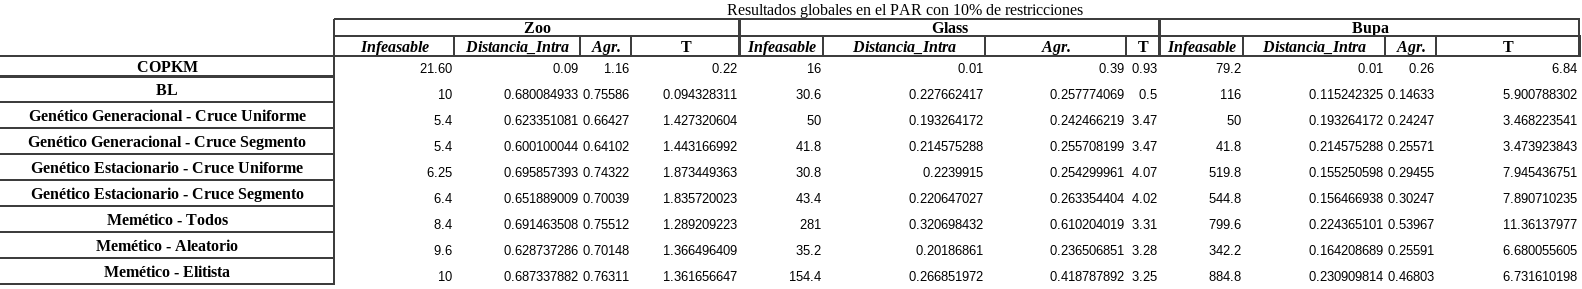
\includegraphics[width=1.0\textwidth]{tablas_globales_10}
    \caption{Tablas Globales - 10\% de restricciones}
\end{figure}

\begin{figure}[H]
    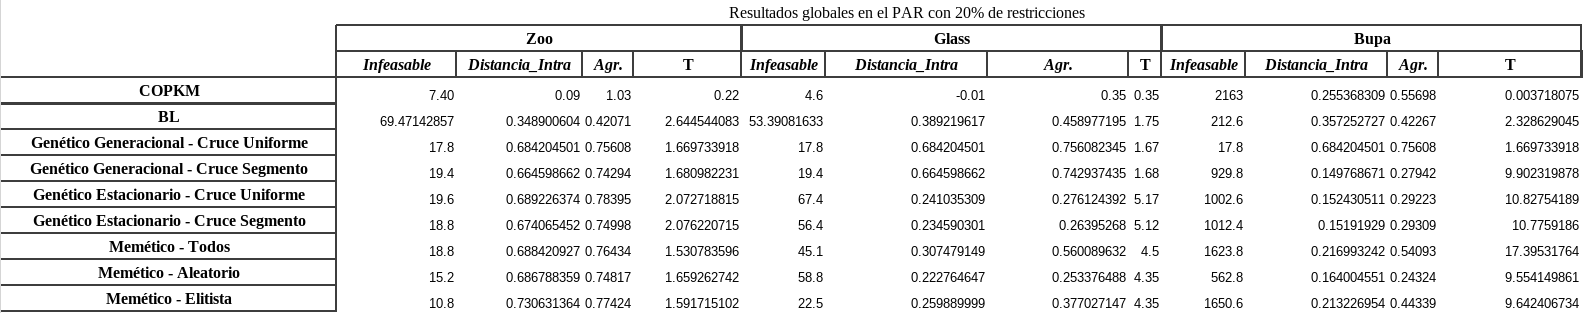
\includegraphics[width=1.0\textwidth]{tablas_globales_20}
    \caption{Tablas Globales - 20\% de restricciones}
\end{figure}

\subsection{Análisis de resultados}

Por las correcciones en la búsqueda local y el algoritmo \emph{greedy}, se puede ver que los resultados respecto a estas dos búsquedas han cambiado respecto la práctica anterior. Estas correcciones se comentan en \emph{\ref{seccion:correcciones}. \nameref{seccion:correcciones}}. Es notorio que, en \emph{Bupa 20\%}, tengamos un tiempo de ejecución tan pequeño. Esto se justifica en la corrección al ver lo que hemos tenido que hacer para poder asignar valor a este \emph{dataset}.

Al tener tanta información condensada en dos tablas, procedemos a comentar los resultados \emph{dataset} a \emph{dataset}, para finalizar tomando conclusiones de estas discusiones.

\subsubsection{Zoo 10\%}

Como era de esperar, \emph{greedy} es el algoritmo que peor \emph{fitness} ha obtenido. La búsqueda local ha sido superada por todos los algoritmos generacionales, salvo el memético elitista.

\subsubsection{Conclusiones}

El algoritmo memético, en alguna de sus variantes, siempre ha sido el que mejores resultados ha obtenido. Dependiendo del \emph{dataset} considerado, el ganador es una u otra variante. Esto es de esperar, pues las distintas variantes establecen distintos equilibrios exploración-explotación, y este equilibrio óptimo puede venir altamente influenciado por el conjunto de datos que queremos resolver.

Es destacado también que en algunos casos, alguna variante memética es peor que los otros algoritmos. Esto puede ser explicado pensando que los algoritmos genéticos, en sus cuatro variantes, también definen su propio equilibrio exploración-explotación, que para ciertos problemas puede ser más acertada que el propuesto por dicho memético con mal comportamiento.

El algoritmo memético elitista está generando resultados malos de forma consistente, en comparación a la búsqueda local y el resto de genéticos y meméticos. A compañeros nuestros les ofrecen resultados mucho mejores, lo que nos hace pensar que hemos cometido un error en la práctica. Este error puede venir dado por:

\begin{itemize}
    \item Durante toda la práctica hemos tenido problemas con la diversidad en la población. Si este problema ha persistido sin tener mucho impacto en el resto de algoritmos, en el elitista se puede ampliar. Esto porque estamos haciendo más grande la diferencia entre individuos de buen \emph{fitness} e individuos de mal \emph{fitness}
    \item En la selección del mejor individuo, usamos una cola con prioridad. Puede ser que nos esté devolviendo los peores elementos, en vez de los mejores.
\end{itemize}

El problema era el segundo. Cambiamos el código y repetimos las ejecuciones, para \lstinline{memeelitist}. No podemos guardar la traza y depurarla de nuevo con el poco tiempo del que disponemos, así que directamente mostramos los resultados en la siguientes tablas:



\pagebreak

\section{Correcciones respecto la práctica pasada} \label{seccion:correcciones}

\begin{itemize}
    \item En la búsqueda local, en vez de considerar iteraciones, consideramos el máximo de evaluaciones del fitness
    \item En la búsqueda local, en vez de considerar iteraciones, consideramos el máximo de evaluaciones del fitness
    \item Hemos puesto finalmente la solución de \emph{Copkmeans} para \emph{Bupa 20\%} en las tablas
\end{itemize}

Estas correcciones no las plasmamos en el pseudocódigo, pues pensamos que es lo lógico al no ser esta parte evaluada de nuevo en esta práctica. Realizamos las correcciones para que las comparaciones entre distintos algoritmos sean lo más justas posbile.

El problema que teníamos con \emph{greedy}, no es que en algún momento alcanzásemos una solución no válida. En ese caso, sería sencillo devolver la última solución válida alcanzada. El problema es que no éramos capaces de generar ni una sola solución valida. Para solucionar esto, en el caso de \emph{Bupa 20\%}, y \textbf{únicamente en ese caso}, hemos empleado el siguiente código para obtener al menos unos valores:


\begin{lstlisting}[language=Rust, style=Boxed]
for i in 0..data_points.len(){
    current_cluster_indixes[i as usize] = (i % number_of_clusters as usize) as u32;
}
let curr_sol = Solution::new(
    current_cluster_indixes.clone(),
    data_points,
    constraints,
    number_of_clusters,
);

return (Some(curr_sol), fitness_evolution);
\end{lstlisting}

Construimos una solución cíclica y devolvemos esa como resultado, que claramente será válida.

\end{document}
